\documentclass[11pt]{report}
\usepackage[utf8]{inputenc}
\usepackage{graphicx}
\usepackage{lipsum}
\usepackage[noindentafter]{titlesec}
\usepackage{sectsty,textcase}
\usepackage{titlesec}
\usepackage{mathptmx}
\usepackage{acro}

\usepackage[T1]{fontenc}
\usepackage{booktabs}
\usepackage{tabularx}
\usepackage[table]{xcolor}
\usepackage{amsmath}
\renewcommand\tabularxcolumn[1]{m{#1}}

\usepackage[left=3cm,right=3cm,top=3cm,bottom=3cm,]{geometry}

\usepackage{enumitem}
\setlist[description]{style=nextline}

\usepackage[
    urldate=long,		    % default: short, e.g. 08/15/2010
    style=authoryear-icomp,	% Harvard citation style
    sorting=nty,            % this is default: sort by name, title, year
    style=apa,
    backend=biber,
    language=english,
    sortlocale=de-DE,    % set according to your needs
    natbib=true,		    % if you want to use natbib compatible citation commands; do _not_ use package natbib!
    maxbibnames=1000,
]{biblatex}
\addbibresource{references.bib}

\usepackage{hyperref}

\usepackage{datetime2}

% contend driven package
\RequirePackage{listings}
\RequirePackage{algorithm2e}
\RequirePackage[record=only,acronym,nonumberlist,nopostdot=false,toc=true]{glossaries-extra} % provides extra glossaries features plus bib2gls, use convertgls2bib  defns.tex defns.bib to convert

\newcommand\docversion{DRAFT \today\hspace{0.1cm}\DTMcurrenttime}


\renewenvironment{abstract}
 {\par\noindent{KURZFASSUNG: }\ \ignorespaces}
 {\par\medskip}

% if not used with overleaf add data input here
% if not using overleaf - data is needed separately
\newcommand{\typeOfWork}{Master Thesis}
\newcommand{\titleToObtain}{Master of Science in Engineering}
\newcommand{\studyProgram}{Master Program Cloud Computing Engineering}
\newcommand{\yourNameInclTitle}{Akademische(r) Grad(e)  Vorname Zuname}
\newcommand{\yourMatNumber}{12345678}
\newcommand{\supervisorNameInclTitle}{Akademische(r) Grad(e)  Vorname Zuname}
\newcommand{\departmentName}{Department Informationstechnologie und Informationsmanagement}
\newcommand{\yourThesisTitle}{Please enter your Thesis Title here, up to 70 characters. If necessary, adapt spaces in FHBgld\_Thesis.}
\newcommand{\thesisDate}{March \ordinalnum{17} 2021}
\newcommand{\universityCityCountry}{FH-Burgenland, Eisenstadt, Österreich}
\newcommand{\thesisBookLiteratureLabel}{Literaturverzeichnis}
\hypersetup{
    pdftitle={\yourThesisTitle},
    pdfsubject={\typeOfWork},
    pdfauthor={\yourNameInclTitle},
    breaklinks, % permits line breaks for long links
    bookmarksnumbered,        % ... and include section numbers
    linktocpage,        % "make page number, not text, be link on TOC ..."
    colorlinks,            % yes ...
    linkcolor=black,        % normal internal links;
    anchorcolor=black,   
    citecolor=black,
    urlcolor=blue,        % quite common
    pdfstartview={Fit},        % "Fit" fits the page to the window
    pdfpagemode=UseOutlines,    % open bookmarks in Acrobat
    plainpages=false      % avoids duplicate page number problem
}

\begin{document}
\pagestyle{empty}
\pagenumbering{gobble}

\begin{flushleft}
    \LARGE{\yourThesisTitle}
\end{flushleft}
\subsectionfont{\fontsize{13}{16}\normalfont}
\titlespacing\subsection{0pt}{0ex}{0ex}
\subsection*{\yourNameInclTitle}
\vspace{-0.5em}
\noindent{\textit{\universityCityCountry}}

% define header appearance
\titleformat{\chapter}{\normalfont\large}{\thechapter}{20pt}{\normalfont\large\MakeUppercase}
\chapterfont{\fontsize{13}{16}\normalfont\MakeUppercase}
\titlespacing\chapter{0pt}{2ex}{2ex}
\sectionfont{\fontsize{13}{16}\normalfont}
\titlespacing\section{0pt}{0ex}{0ex}
\subsectionfont{\fontsize{13}{16}\normalfont}
\titlespacing\subsection{0pt}{0ex}{0ex}
\subsubsectionfont{\fontsize{13}{16}\normalfont}
\titlespacing\subsection{0pt}{0ex}{0ex}
% numbering subsubsections
\setcounter{secnumdepth}{5}

% do not start chapter on new page
\makeatletter
\patchcmd{\chapter}{\clearpage}{\leavevmode\flushleft}{}{}
\makeatother

\vspace{5em}
\begin{abstract}
    Der Leser der Kurzfassung soll verstehen, welche Problemstellung / Fragestellung durch die vorliegende Arbeit bearbeitet wird und welche Erkenntnisse und Ergebnisse vorliegen.

\end{abstract}
\vspace{2em}

\chapter{Introduction}
Welcome to the \LaTeX{} template prepared for the Computer Science department at the university of applied sciences of Burgenland\footnote{\url{https://www.fh-burgenland.at/en/information-technology/about-the-department/}}. 

Introduction, Problem, Objective, Demarcation, Question, Method, and a description of the overall structure should go into this chapter.

\section{Instruction included in the original FHBgld word processor template}
In der Problemstellung erfolgt eine Hinführung zum Thema aus dem globalen
Zusammenhang heraus betrachtet: Warum es wichtig ist, sich mit dem konkreten
Thema zu beschäftigen bzw. welche Bedeutung hat dieses Thema zum Beispiel für die
Wirtschaft, Gesellschaft und Umwelt.

\section{Using the \LaTeX{} template}

Everything in the template revolves around the\verb|main.tex| file. Here all the other files are put together to create the thesis.
There are three different sections to consider: 
\begin{itemize}
	\item Front Matter,
	\item Chapters, and
	\item Back Matter.
\end{itemize}
Each section has a folder where you can put the different parts of your thesis. In the Front Matter section you should put everything that comes before your first chapter of the thesis. Respectively, in the Back Matter section you put everything that comes after your last chapter. And finally all the chapters are put into the Chapters folder. You can put things like abstract, summaries, etc... wherever they suit your thesis. In the end it really only matters how you add them into your \verb|main.tex| file. With the \verb|\input{}| command you can add the parts if they should appear in your thesis, the order within the \verb|main.tex| also determines the order in the final pdf.

\subsection{Title-page}
The Layout of the Title-page is in the \verb|FHBgld_Thesis.cls|, normally it remains unchanged. You can use all the commands as seen in the \verb|Titlepage.tex|. 

The template and also the titlepage is based on the scrbook class. So if you want to use a different class without changing the title page in the \verb|FHBgld_Thesis.cls|, it is recommended creating the title page separately and then include the compiled pdf file here, using the 
\verb|\includepdf{<filename>}| from the \verb|pdfpages| package. Alternatively, you may use the word template for the title- page and add it using this package. In that way you can avoid any differences to the original title page template. The word templates can be found here:
\begin{enumerate}
	\item \url{https://moodle.fh-burgenland.at/pluginfile.php/34046/mod_folder/content/0/03_Vorlage_zur_Erstellung_wissenschaftlicher_Arbeiten\%20V2.8.docx?forcedownload=1}
	\item \url{https://moodle.fh-burgenland.at/pluginfile.php/34046/mod_folder/content/0/03_Vorlage_zur_Erstellung_wissenschaftlicher_Arbeiten\%20V2.8\%20eng.docx?forcedownload=1}
\end{enumerate}

If you use the \verb|includepdf| package make sure that the pdf still has the correct metadata afterwards.

\subsection{Citing}
As per requirement of the FH Burgenland, the template class is configured for APA\footnote{\url{https://ctan.org/pkg/biblatex-apa?lang=en}} style: \verb|[natbib=true, backend=biber, style=apa, sorting=nty]|. It uses Biblatex and the Biber backend. The location of the bibliography file is defined in the \verb|main.tex|. Citation xamples:
\begin{itemize}
	\item \verb|\parencite{bibid}| provides \parencite{lamport94}
	\item \verb|\parencite[p. 123ff]{bibid}| provides \parencite[p. 123ff]{lamport94}
	\item \verb|\parencite{lamport94,talbot2013using}| provides \parencite{lamport94,talbot2013using}
\end{itemize}

\subsection{Temporary packages and settings}
Some packages and settings are included to make creating your thesis easier, e.g. FixMe.
Before building your final PDF, those should be removed. Use \verb|grep -r RMF *| in the root folder of the template to find the packages and settings that should be removed.

\section{Creating the pdf}
To create a proper pdf file of your thesis there are some things to consider

\subsection{PDF build}
The script \verb|build.sh| is provided to compile the thesis in four steps:
\begin{enumerate}
	\item pdflatex main.tex
	\item biber main
	\item bib2gls main
	\item pdflatex main.tex
\end{enumerate}
\verb+bib2gls+ is used to prepare the indexes for glossaries and acronyms. Both are edited in \verb|defns.bib|, therefore, Jabref can be used to manage entries. 

In case you already have your definitions in \LaTeX{} format, such as
\begin{itemize}
	\item \verb|\newacronym{gcd}{GCD}{Greatest Common Divisor}}|, or
	\item \verb|\newglossaryentry{latex}{name=latex,description={Is a mark up language specially suited for scientific documents}}|
\end{itemize}
use \verb|convertgls2bib defns.tex defns.bib| to convert from \LaTeX{} to Bibtex.

\subsection{Embed all fonts in pdf}
Please make sure that you embed all fonts in your pdf. Also make sure all the fonts of any figures that were used in the document are embedded. 
If you don't use any pdf figures, pdfLaTeX should embed all fonts automatically.

\subsubsection{Linux}
On Linux you can use the command \begin{verbatim}
	pdffonts my_file.pdf
\end{verbatim}
to check if the fonts are embbeded. Check if all the fonts listed have a "yes" in the "emb" column. 
\begin{verbatim}
name                                 type              encoding         emb sub uni 
------------------------------------ ----------------- ---------------- --- --- --- 
BXJBCJ+NimbusSanL-Bold               Type 1            Custom           yes yes no     
HEMYJL+NimbusSanL-Regu               Type 1            Custom           yes yes no     
OOJWDR+SFRM1000                      Type 1            Custom           yes yes no      
OHLNOC+SFRM0900                      Type 1            Custom           yes yes no   
...
\end{verbatim}
For more information see 

\url{https://www.karlrupp.net/2016/01/embed-all-fonts-in-pdfs-latex-pdflatex/}
\subsubsection{Windows}
On Windows using the Adobe Acrobat Reader the fonts can be found at
\begin{verbatim}
	File > Properties > Fonts
\end{verbatim}
For more information please consult
\begin{enumerate}
	\item \url{https://helpx.adobe.com/acrobat/using/pdf-fonts.html}
	
	\item \url{https://www.overleaf.com/learn/latex/Questions/My_submission_was_rejected_by_the_journal_because_%22Font_XYZ_is_not_embedded%22._What_can_I_do%3F} 
	\end{enumerate}
	
	%\subsection{Making a PDF/A-1 compatible pdf}
	\subsection{Making a PDF}

	
	\subsubsection{validation}
	To validate the produced PDF, you can either use the Preflight tool included in Adobe Acrobat Pro or a free online version. E.g. \url{https://www.pdf-online.com/osa/validate.aspx}.
	Please take caution as different validation tools can report different results.
	
	\subsubsection{metadata}
	There may be a section in the beginning of a .tex file where you define metadata.
	Setting your Name, Title, Subject, Keywords and remove/add Information for example. To find out what fields are possible please check here. \url{http://texdoc.net/texmf-dist/doc/latex/pdfx/pdfx.pdf#subsection.2.3}
	
	A file containing the metadata (jobname.xmpdata) is created when compiling. 
	
	Watch out, the metadata .xmpdata file is only created one time. So if you need to update it you need to clear the cache of overleaf. Or delete the .xmpdata file. It is then recreated the next time you compile. 
	
	\url{https://www.overleaf.com/learn/how-to/Clearing_the_cache}
	
	You can check the metadata of your PDF with Acrobat Reader by going to File-> properties. Or alternatively check it with an online tool.
	
	\subsubsection{figures}
	As already mentioned, make sure that all the fonts used in the pictures are included. Furthermore transparency in pictures causes issues, please convert transparent figures into their nontransparent version. 
	
	Using Linux the command \verb|pdfimages -list <pdf>| shows the typpe of all images used. The type should always be \verb|image| and not \verb|smask|. Check and convert these images.
	
	\subsubsection{color}
	Additionally, there can be problems if figures use different color spaces. Use the same command as before and check if all images use the same color. 
	
	If color is really important in your work it might also be a good idea to use an ICC profile for the color. 
	For more details about colors check \url{http://texdoc.net/texmf-dist/doc/latex/pdfx/pdfx.pdf#subsection.2.5}
	
	It is also possible to convert the pictures automatically using ghostscript. But always check the results manually. 
	
	\subsubsection{Other errors}
	Due to the complexity of Latex files there can be many more errors that are not covered here.
	
	The Preflight tool included in Adobe Acrobat Pro also has the ability to fix some errors. For example EOL (End of Line) errors can be fixed with its analyize and fix option. 
	Please also check if any of the following pages might have a solution to your problem:
	\begin{enumerate}
		\item \url{https://www.mathstat.dal.ca/~selinger/pdfa/}
		\item \url{https://blog.zhaw.ch/icclab/creating-pdfa-documents-for-long-term-archiving/}
		\item german: \url{http://kulturreste.blogspot.com/2014/06/grrrr-oder-wie-man-mit-latex-vielleicht.html}
		\item \url{https://support.stmdocs.in/wiki/?title=Generating_PDF/A_compliant_PDFs_from_pdftex}
		\item \url{http://texdoc.net/texmf-dist/doc/latex/pdfx/pdfx.pdf}
	\end{enumerate}
	
	\subsubsection{Tagged PDF}
	Currently with Latex it is only possible to create files that are in the PDF/A-1b format. The PDF/A-1a format required the PDF to be tagged which is currently not possible in a satisfactory way.
	A manual tagging with Adobe Acrobat Pro is possible but not recommended.
	
	More information about the current status of tagged pdfs can be found here:
	\begin{enumerate}
		\item \url{https://umij.wordpress.com/2016/08/11/the-sad-state-of-pdf-accessibility-of-latex-documents/} 
		\item \url{https://www.tug.org/TUGboat/tb30-2/tb95moore.pdf}
	\end{enumerate}
	
	\subsection{General Remarks to create the pdf}
	Highest priority should always be the embedding of all fonts. Further compliance with the PDF/A standards is always desired, but talk to your advisor in any case.
	
	Please also check the following resources if you have problems and need assistance
	
	\begin{enumerate}
		\item \url{https://spl29.univie.ac.at/fileadmin/user_upload/s_spl29/Studium/abschluss_master/Infoblatt_Hochschulschriften.pdf} 
		\item \url{https://e-theses.univie.ac.at/E-Theses_erstellen_von_pdf.pdf}
	\end{enumerate}
	
	\section{Further tips on the template}
	In the following chapters there are some general tips on the elements of Latex. You can check them out if you think they have useful information for you. Then you delete these chapters and replace them with the real chapters of your thesis.

\chapter{Fundamentals} 	% Produces section heading.  Lower-level

Basics such as theory, definitions, relevant theories, related work and state of the art should be included here.

\section{Instruction included in the original FHBgld word processor template}
\subsection{General definitions}
Die in dieser Formatvorlage beispielhaft enthaltenen Überschriften sind auf die im
konkreten Fall tatsächlich passenden Überschriften anzupassen.
In diesem Teil der Arbeit werden die zum eindeutigen Verständnis unbedingt
erforderlichen Grundlagen und Definitionen sowie die Erklärung wichtiger Begriffe
angeführt.
Die Gliederungspunkte müssen möglichst prägnant bezeichnet werden.
\subsection{Related work / state of research}
Auch die neuesten Entwicklungen und Arbeiten auf diesem Gebiet (Stand der
Wissenschaft oder auch state-of-the-art) sind darzulegen, wobei diese je nach Thema
auch in der 1. Gliederungsebene behandelt werden können.

\section{Ordinary text}
% A '%' character causes TeX to ignore all remaining text on the line,
% and is used for comments like this one.

% sections are begun with similar 
% \subsection and \subsubsection commands.

The ends  of words and sentences are marked by spaces. It doesn't matter how many 
spaces    you type; one is as good as 100.  The
end of   a line counts as a space.

One   or more   blank lines denote the  end 
of  a paragraph.  

Since any number of consecutive spaces are treated
like a single one, the formatting of the input
file makes no difference to
\LaTeX,                % The \LaTeX command generates the LaTeX logo.
but it makes a difference to you.  When you use 
\LaTeX \cite{lamport94},  % \cite inserts a reference, which you define at the end of the document
making your input file as easy to read
as possible will be a great help as you write 
your document and when you change it.  This sample 
file shows how you can add comments to your own input 
file.

Because printing is different from typewriting,
there are a number of things that you have to do
differently when preparing an input file than if
you were just typing the document directly.
Quotation marks like
``this'' 
have to be handled specially, as do quotes within
quotes:
``\,`this'            % \, separates the double and single quote.
is what I just 
wrote, not  `that'\,''.  

Dashes come in three sizes: an 
intra-word 
dash, a medium dash for number ranges like 
1--2, 
and a punctuation 
dash---like 
this.

A sentence-ending space should be larger than the
space between words within a sentence.  You
sometimes have to type special commands in
conjunction with punctuation characters to get
this right, as in the following sentence.
Gnats, gnus, etc.\ all  % `\ ' makes an inter-word space.
begin with G\@.         % \@ marks end-of-sentence punctuation.
You should check the spaces after periods when
reading your output to make sure you haven't
forgotten any special cases.  Generating an
ellipsis
\ldots\               % `\ ' is needed after `\ldots' because TeX 
% ignores spaces after command names like \ldots 
% made from \ + letters.
%
% Note how a `%' character causes TeX to ignore 
% the end of the input line, so these blank lines 
% do not start a new paragraph.
%
with the right spacing around the periods requires
a special command.

\LaTeX\ interprets some common characters as
commands, so you must type special commands to
generate them.  These characters include the
following:
\$ \& \% \# \{ and \}.

In printing, text is usually emphasized with an
\emph{italic}  
type style.  

\begin{em}
	A long segment of text can also be emphasized 
	in this way.  Text within such a segment can be 
	given \emph{additional} emphasis.
\end{em}

It is sometimes necessary to prevent \LaTeX\ from
breaking a line where it might otherwise do so.
This may be at a space, as between the ``Mr.''\ and
``Jones'' in
``Mr.~Jones'',        % ~ produces an unbreakable interword space.
or within a word---especially when the word is a
symbol like
\mbox{\emph{itemnum}} 
that makes little sense when hyphenated across
lines.

Footnotes\footnote{This is an example of a footnote.}
pose no problem.

\LaTeX\ is good at typesetting mathematical formulas
like
\( x-3y + z = 7 \) 
or
\( a_{1} > x^{2n} + y^{2n} > x' \)
or  
\( AB  = \sum_{i} a_{i} b_{i} \).
The spaces you type in a formula are 
ignored.  Remember that a letter like
$x$                   % $ ... $  and  \( ... \)  are equivalent
is a formula when it denotes a mathematical
symbol, and it should be typed as one.
Furthermore you can add a formula as Images or Tables, see Formula  \hyperref[eq:abc]{\ref{eq:abc}}
\begin{equation}
	\label{eq:abc}
	a+b=c
\end{equation}

It is sometimes necessary to prevent \LaTeX\ from
breaking a line where it might otherwise do so.
This may be at a space, as between the ``Mr.''\ and
``Jones'' in
``Mr.~Jones'',        % ~ produces an unbreakable interword space.
or within a word---especially when the word is a
symbol like
\mbox{\emph{itemnum}} 
that makes little sense when hyphenated across
lines.
\chapter{Methodology}

Approach, methods, and objectives should come here.

\section{Instruction included in the original FHBgld word processor template}
\subsection{Approach}
Alle im durchgeführten Untersuchungen und Versuche müssen systematisch und
nachvollziehbar sein. Daher ist die gewählte Vorgangsweise genau zu beschreiben
und zu begründen. Es empfiehlt sich, dafür Literatur zum wissenschaftlichen Arbeiten
heranzuziehen.
\subsection{Research methods}
Die eingesetzte Methoden (z.B. Online-Befragung, Inhaltsanalyse, Interviews) müssen
ebenfalls nachvollziehbar beschrieben werden.
Unterschiedliche Untersuchungsmethoden haben oft unterschiedliche Genauigkeit.
Neben der Begründung und Beschreibung der Untersuchungsmethoden ist auch eine
Begründung und Beschreibung der verwendeten Auswertungsmethoden bzw. dafür
verwendete Software unerlässlich\footnote{Wenn der Abstand zwischen Fußnotentrennstrich und Fußnote zu groß wird, gehen Sie folgend vor:
	Wählen Sie im Hauptmenü „Ansicht | Entwurf | Verweise | Notizen anzeigen |
	Fußnotentrennlinie". Dann können Sie unnötige Leerzeichen entfernen.
}.
Wenn es ein Kapitel 3.2.1 gibt, muss es auch ein Kapitel 3.2.2 geben.

\subsubsection{<<Überschrift 4. Ebene>>}
4 Überschriftenebenen müssen reichen.


\section{Displayed Text}
Text is displayed by indenting it from the left
margin.  Quotations are commonly displayed.  There
are short quotations
\begin{quote}
	This is a short quotation.  It consists of a 
	single paragraph of text.  See how it is formatted.
\end{quote}
and longer ones.
\begin{quotation}
	This is a longer quotation.  It consists of two
	paragraphs of text, neither of which are
	particularly interesting.
	
	This is the second paragraph of the quotation.  It
	is just as dull as the first paragraph.
\end{quotation}
Another frequently-displayed structure is a list.
The following is an example of an \emph{itemized}
list.
\begin{itemize}
	\item This is the first item of an itemized list.
	Each item in the list is marked with a ``tick''.
	You don't have to worry about what kind of tick
	mark is used.
	
	\item This is the second item of the list.  It
	contains another list nested inside it.  The inner
	list is an \emph{enumerated} list.
	\begin{enumerate}
		\item This is the first item of an enumerated 
		list that is nested within the itemized list.
		
		\item This is the second item of the inner list.  
		\LaTeX\ allows you to nest lists deeper than 
		you really should.
	\end{enumerate}
	This is the rest of the second item of the outer
	list.  It is no more interesting than any other
	part of the item.
	\item This is the third item of the list.
\end{itemize}
You can even display poetry.
\begin{verse}
	There is an environment 
	for verse \\             % The \\ command separates lines
	Whose features some poets % within a stanza.
	will curse.   
	
	% One or more blank lines separate stanzas.
	
	For instead of making\\
	Them do \emph{all} line breaking, \\
	It allows them to put too many words on a line when they'd rather be 
	forced to be terse.
\end{verse}

Mathematical formulas may also be displayed.  A
displayed formula 
is 
one-line long; multiline
formulas require special formatting instructions.
\[  \Gamma \times  \psi = x'' + y^{2} + z_{i}^{n}\]
Don't start a paragraph with a displayed equation,
nor make one a paragraph by itself.

\chapter{Empirical work}

\section{Instruction included in the original FHBgld word processor template}
Die Durchführung der empirischen Untersuchung ist nachvollziehbar zu dokumentieren sowie auch die dabei aufgetretenen Probleme und deren Behandlung. Der Umfang ergibt sich aus der Art der Bearbeitung.  

Tabelle 1 zeigt ein Bespiel für eine Tabelle. 

\begin{figure}[ht]
	\centering
	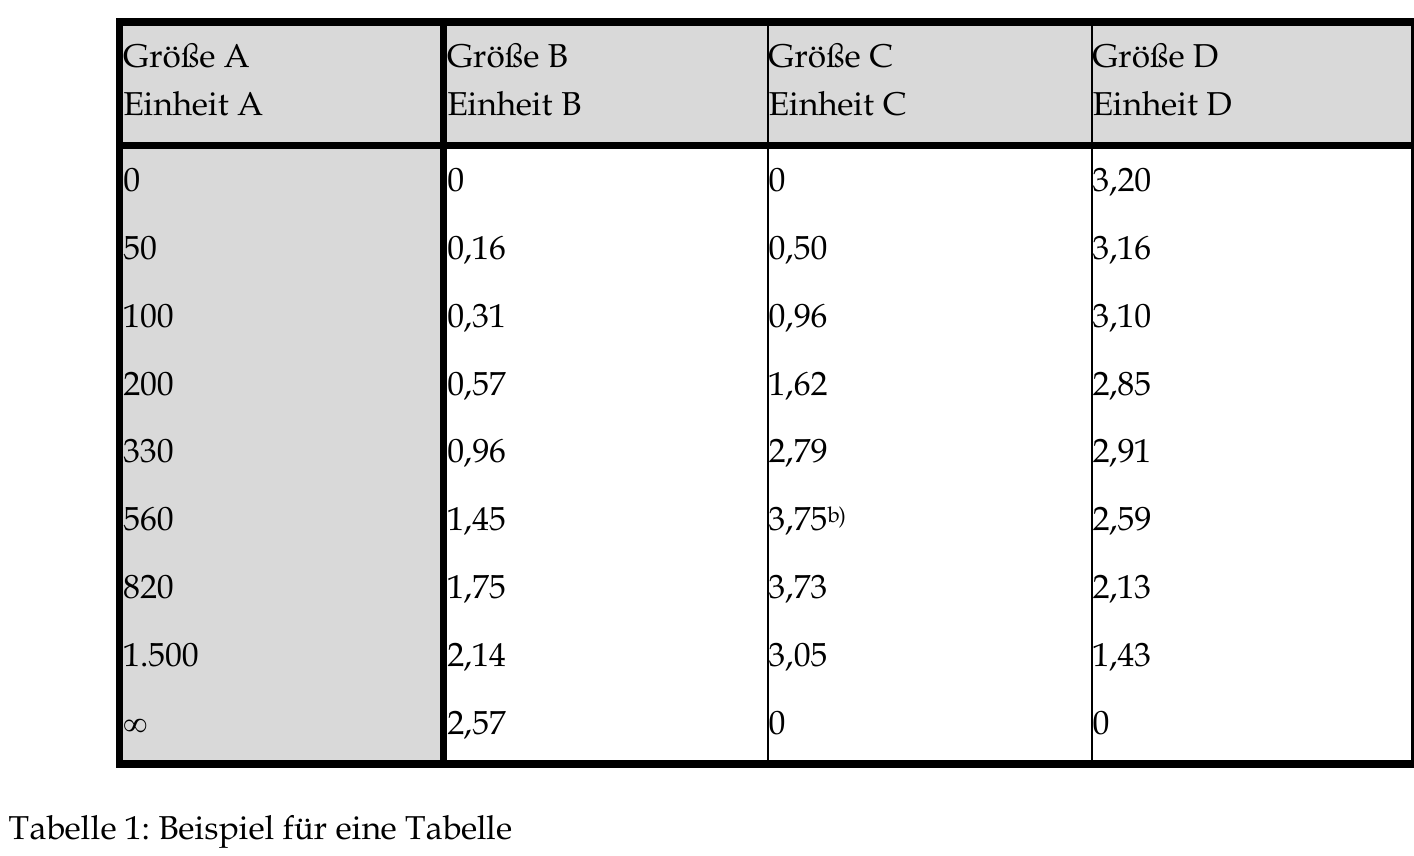
\includegraphics[width=0.7\linewidth]{figures/Word_Table}
	\caption{Screenshot example from FHBgld word processor template}
	\label{fig:wordtable}
\end{figure}
Abbildung 1 zeigt ein Beispiel für eine Abbildung oder Grafik.
\begin{figure}
	\centering
	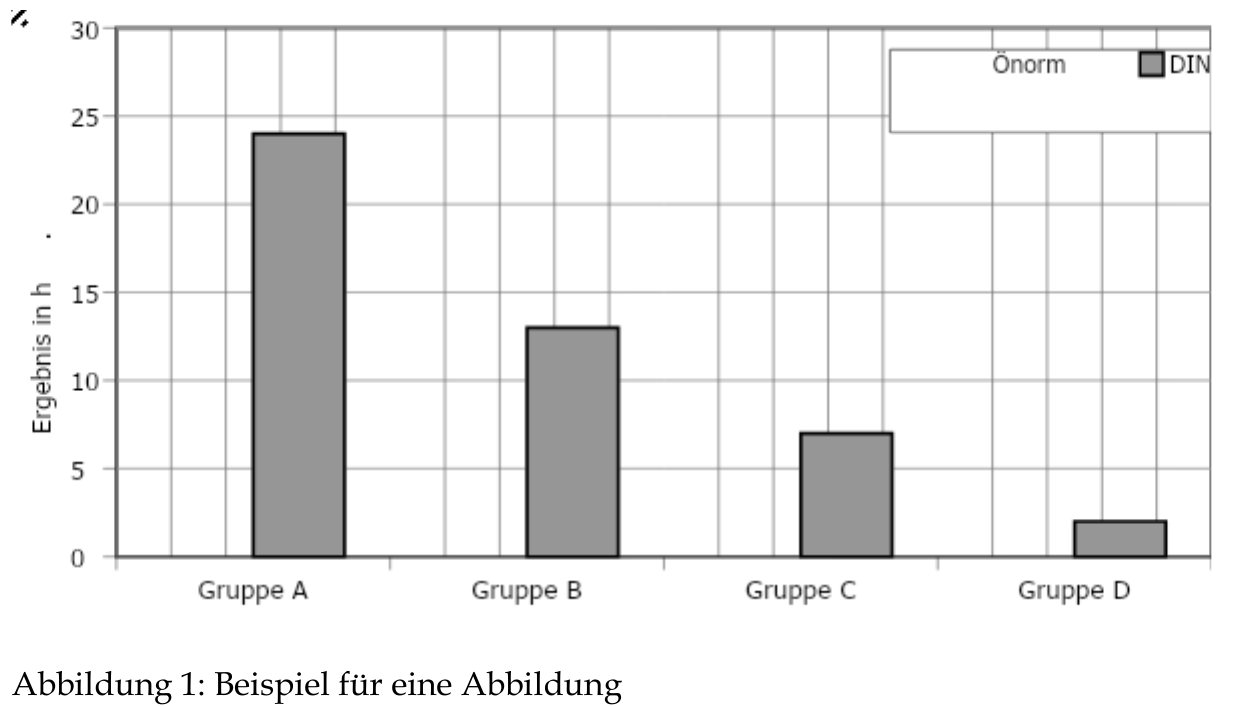
\includegraphics[width=0.7\linewidth]{figures/Word_Diagram}
	\caption{Screenshot example from FHBgld word processor template}
	\label{fig:worddiagram}
\end{figure}
\linebreak
Mathematisch werden die Zusammenhänge wie im Figure \ref{fig:wordformel} beschrieben.
\begin{figure}
	\centering
	
\includegraphics[width=0.7\linewidth]{figures/Word_Formel}
	\caption{Screenshot example from FHBgld word processor template}
	\label{fig:wordformel}
\end{figure}

\section{Tables and Images with \LaTeX}
One of the great advantages of \LaTeX{} is that all it needs to know is
the structure of a document, and then it will take care of the layout
and presentation itself.  So, here we shall begin looking at how exactly
you tell \LaTeX{} what it needs to know about your document.

\subsection{Tables}
In this sub-section, a simple table is inserted. To add reference to the table, see (cf. Table~\hyperref[tab:tableexample0]{\ref{tab:tableexample0}}):

%A simple table.  The center environment is first set up, otherwise the
%table is left aligned.  The tabular environment is what tells Latex
%that the data within is data for the table.
% https://en.wikibooks.org/wiki/LaTeX/Tables
\begin{table}[htb]
	\begin{tabular}{|b{7cm}|c|}
		%The tabular environment is what tells Latex that the data within is
		%data for the table.  The arguments say that there will be two
		%columns, both left justified (indicated by the 'l', you could also
		%have 'c' or 'r'.  The bars '|' indicate vertical lines throughout
		%the table.
		
		\hline  % Print horizontal line
		\fontsize{11pt}{12pt}\selectfont Command & Level \\ \hline  % Columns are delimited by '&'.  And
		%rows are delimited by '\\'
		\fontsize{10pt}{14pt}\selectfont Some sections to provide some examples: & \\
		\texttt{\textbackslash part\{\emph{part}\}} & -1 \\
		\texttt{\textbackslash chapter\{\emph{chapter}\}} & 0 \\
		\texttt{\textbackslash section\{\emph{section}\}} & 1 \\
		\texttt{\textbackslash subsection\{\emph{subsection}\}} & 2 \\
		\texttt{\textbackslash subsubsection\{\emph{subsubsection}\}} & 3 \\
		\texttt{\textbackslash paragraph\{\emph{paragraph}\}} & 4 \\
		\texttt{\textbackslash subparagraph\{\emph{subparagraph}\}} & 5 \\
		\hline
		
	\end{tabular}
	\caption{some description of the table}
	\label{tab:tableexample0}
\end{table}

\subsubsection{More tabular examples}

First, a plain simple example for a FHBgld table, see table~\hyperref[tab:tab:tableexample1]{\ref{tab:tableexample1}}.

\begin{table}[h]
	\centering
	\begin{tabular}{|b{1cm}|b{2cm}|b{3cm}|b{4cm}|}
		\hline
		\multicolumn{4}{|l|}{\fontsize{11pt}{12pt}\selectfont\noindent First line in 11pt fontsize } \\ \hline
		1cm & 2cm & 3cm & 4cm \\ \hline
		from & here on & the table & font size \\ \hline
		will & be as & defined & in class, that is 10pt\footnote{yes, really!} \\ \hline
		will & be as & defined & in class, that is 10pt\footnote{yes, really!} \\ \hline
		will & be as & defined & in class, that is 10pt\footnote{yes, really!} \\ \hline
		will & be as & defined & in class, that is 10pt\footnote{yes, really!} \\ \hline
		will & be as & defined & in class, that is 10pt\footnote{yes, really!} \\ \hline
	\end{tabular}
	\caption{some description of the table}
\label{tab:tableexample1}
\end{table}

Next, a table with nine columns, see table~\hyperref[tab:tableexample2]{\ref{tab:tableexample2}}.

\begin{table}[h]
	\centering
	\begin{tabular}{|*{9}{l|}}
		\hline
		{\fontsize{11pt}{12pt}\selectfont This} & {\fontsize{11pt}{12pt}\selectfont table} & {\fontsize{11pt}{12pt}\selectfont has} & {\fontsize{11pt}{12pt}\selectfont way} & {\fontsize{11pt}{12pt}\selectfont too } & {\fontsize{11pt}{12pt}\selectfont many} & {\fontsize{11pt}{12pt}\selectfont columns}, & {\fontsize{11pt}{12pt}\selectfont does'nt} & {\fontsize{11pt}{12pt}\selectfont it?} \\ \hline
		One & Two & Three & Four & Five & Six & Seven & Eight & Nine! \\ \hline
		At & least & the & first & column & has & 11pt & font & size. \\ \hline
	\end{tabular}
	\caption{some description of the table}
	\label{tab:tableexample2}
\end{table}

\subsection{Images}
% Here is how to insert an image as a figure. There is a lot more you can do
% when inserting images, check out: https://en.wikibooks.org/wiki/LaTeX/Importing_Graphics

\begin{figure}[h]
	\centering
	
\includegraphics[width=0.3\textwidth]{figures/logo_nontransparent.jpg}
	\caption{Image Example}
	\label{fig:image_example}
\end{figure}

When an image is inserted, you can refer to it like this (cf. Figure~\hyperref[fig:image_example]{\ref{fig:image_example}}).

\subsubsection{A Subsubsection}
As one last example, this is how you can insert a sub-sub-section! Have fun
writing your thesis with \LaTeX{}!

\lipsum[2-3]
\raggedbottom

\pagebreak

\chapter{Discussion of results and conclusions}

Results, Discussion and conclusions come here.

\section{Instruction included in the original FHBgld word processor template}
Die Ergebnisse der Arbeit sind in übersichtlicher Form darzustellen Die gewählte Form der Darstellung ist vom gewählten Datenmaterial und den in der Einleitung gesetzten Zielen abhängig. Die Ergebnisse sind zu interpretieren und in Bezug zum Stand des Wissens zu diskutieren. Über die Beantwortung der Forschungsfrage und die daraus gezogenen Schlussfolgerungen schließt sich der Bogen zur Einleitung. 

Wichtig ist die gedanklich klare Unterscheidung zwischen der Darstellung der Ergebnisse und der Interpretation/Bewertung der Ergebnisse. 

\section{Code}
If you want to show program code within your thesis you can use the \verb|\texttt{verbatim}| environment or for a more complex display take a look at \url{https://www.overleaf.com/learn/latex/Code_listing}

\begin{verbatim}
	Text enclosed inside \texttt{verbatim} environment 
	is printed directly 
	and all \LaTeX{} commands are ignored.
\end{verbatim}

\begin{lstlisting}[language=Python, caption=Python example]
	import numpy as np
	
	def incmatrix(genl1,genl2):
	m = len(genl1)
	n = len(genl2)
	M = None #to become the incidence matrix
	VT = np.zeros((n*m,1), int)  #dummy variable
	
	#compute the bitwise xor matrix
	M1 = bitxormatrix(genl1)
	M2 = np.triu(bitxormatrix(genl2),1) 
	
	for i in range(m-1):
	for j in range(i+1, m):
	[r,c] = np.where(M2 == M1[i,j])
	for k in range(len(r)):
	VT[(i)*n + r[k]] = 1;
	VT[(i)*n + c[k]] = 1;
	VT[(j)*n + r[k]] = 1;
	VT[(j)*n + c[k]] = 1;
	
	if M is None:
	M = np.copy(VT)
	else:
	M = np.concatenate((M, VT), 1)
	
	VT = np.zeros((n*m,1), int)
	
	return M
\end{lstlisting}

\chapter{Synopsis}

\section{Instruction included in the original FHBgld word processor template}
Die Zusammenfassung stellt die gesamte Arbeit – von der Einleitung bis zu den Ergebnissen - in Kurzform dar. Länge maximal 1,5 - 2 Seiten. 

\section{Algorithms}

If you want to show algorithms in your Thesis take a look at the \url{https://www.overleaf.com/learn/latex/algorithms} page. The \verb|algorithm2e| package is already included in the template. You can list algorithms in the same way as you can list Tables and Figures.

\begin{algorithm}[H]
	\KwData{this text}
	\KwResult{how to write algorithm with \LaTeX2e }
	initialization\;
	\While{not at end of this document}{
		read current\;
		\eIf{understand}{
			go to next section\;
			current section becomes this one\;
		}{
			go back to the beginning of current section\;
		}
	}
	\caption{How to write algorithms}
\end{algorithm}
%\cleardoublepage{}

\section{Acronyms and Glossary.}

if you want to use Acronyms or a Glossary check the page here: \url{https://www.overleaf.com/learn/latex/glossaries}

The \Gls{latex} typesetting markup language is specially suitable 
for documents that include \gls{maths}. are 
rendered properly an easily once one gets used to the commands.

Given a set of numbers, there are elementary methods to compute 
its \glsxtrlong{gcd}, which is abbreviated \glsxtrshort{gcd}. This 
process is similar to that used for the \glsxtrfull{lcm}.

\section{Macros}

You can also add useful packages or macros into the \verb|packages_macros.tex| file to add them to the project.
The packages for algorithms, code or the glossary have already been added there.

\subsection{FixMe}
Another example, the \verb|FixMe| package, is added as well. It allows you or your supervisor to add Meta comments to the document. These comments only appear if you set the draft mode in the \verb|main.tex| file. If you remove or comment the activation of the draft mode you can see your final thesis without comments.

\titleformat{\chapter}{\normalfont\Large}{\thechapter}{20pt}{\normalfont\Large}
\printbibliography[title=\thesisBookLiteratureLabel]
\end{document}
